\documentclass{article}
\usepackage[utf8]{inputenc}

\title{Numerieke modellering en benadering - Practicum 1}
\author{Matko Matić }
\date{April 2020}

\usepackage{natbib}
\usepackage{graphicx}

\begin{document}

\maketitle

\section{Introduction}
Dit is het verslag van het eerse practicum voor het vak Numerieke Modellering en Benadering voor de bachelor Ingenieurswetenschappen aan KU Leuven, richting Computerwetenschappen 


\section{Continue kleinste kwadratenbenadering met Chebyshev veel-termen}

\subsection{Evaluate Chebyshev}




\begin{figure}[h!]
\centering
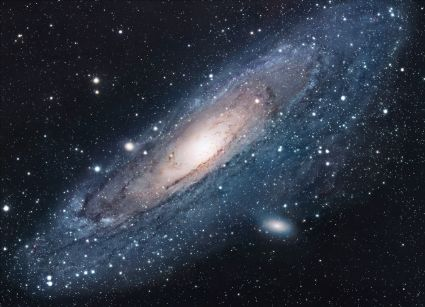
\includegraphics[scale=1.7]{universe}
\caption{The Universe}
\label{fig:universe}
\end{figure}

\section{Conclusion}
``I always thought something was fundamentally wrong with the universe'' \citep{adams1995hitchhiker}

\bibliographystyle{plain}
\bibliography{references}
\end{document}
